\documentclass{article}
\usepackage{a4wide}
\usepackage[utf8]{inputenc}
\usepackage[T1]{fontenc} 
\usepackage{fancyhdr} 
\usepackage{graphicx}
\usepackage{lastpage}
\usepackage{enumerate}
\usepackage{amssymb}
\usepackage{amsmath} 
\usepackage{algorithm}
\usepackage{tikz} 
\usepackage{listings}
\usepackage[noend]{algpseudocode}
\usetikzlibrary{automata, arrows}
\usepackage{subcaption}
\usepackage{hyperref}

\makeatletter
\def\BState{\State\hskip-\ALG@thistlm}
\makeatother



\lhead{
\includegraphics[width=4.6cm]{uni.png}\\ \course\\ \semester\\Project \homeworkNumber}
\rhead{\university\\ \authorname\\\authoremail\\Page \thepage\ of \pageref{LastPage}}

\usepackage[headheight=68pt]{geometry}
\pagestyle{fancy}

%% Custom command
\newcommand{\authorname}{Giorgi Grigalashvili, Fabricio Arend Torres}
\newcommand{\authoremail}{\{g.grigalashvili, fabricio.arendtorres\} @ stud.unibas.ch}
\newcommand{\semester}{Spring Semester 2017}
\newcommand{\course}{Probabilistic Shape Modelling}
\newcommand{\homeworkNumber}{1}

\newcommand{\university}{University of Basel}
\newcommand{\department}{Department of Mathematics and Computer Science}
\newcommand{\address}{Spiegelgasse 1, 4051 Basel, Switzerland}
\newcommand{\website}{dmi.unibas.ch / informatik.unibas.ch}

%% Custom commands

\def\underline#1{\underline{\underline{#1}}}

\begin{document}
	\title{Project 1:\\ Reconstruction of Femurs}
	\begin{abstract}
		In this project, we demonstrate a custom technique for reconstructing 3D femurs using the Scalable Image Analysis and Shape Modelling library Scalismo. 
		A Statistical Shape Model is learned from 50 sample femurs and then augmented with a custom anisotropic kernel. The final SSM is then used for reconstructing 10 femurs with missing parts. 
		The presented reconstruction method does not rely on hand-picked landmarks but instead uses the Iterative Closest Points algorithm.
	\end{abstract}
	
	\section{Introduction}
	
	Modelling of 3D shapes and the reconstruction of missing parts in 3D shapes pose a difficult problem. In this project the goal was reconstructing 10 femurs which were missing different parts. For a reconstruction it is mandatory that the fully reconstructed femur still is a valid femur in the sense that no unnatural deformations are introduced. We target this problem by using the Scalismo library for training a Statistical Shape Model, which can then be fitted onto the incomplete femurs for reconstructing the missing parts.
	
	We present both a method for building a SSM that models natural femurs as well as a method for reconstructing individual incomplete femurs with this SSM.
	

	\section{Method}
	For the reconstruction of incomplete meshes we require a Statistical Shape Model [SSM] that models the variations of femurs appropriately. We use 50 available training femurs for creating a Shape Model that models the variation of the data and augment it with a custom kernel for improving the smoothness.
	
	There are multiple main steps necessary for this approach. 
	First of all, we aligned the training meshes with a reference femur using rigid alignment.
	By doing this, we remove shape variations due to transformation or translation. 
	The next step is creating a SSM, which models the variations of the different training femurs.
	The SSM is a gaussian process, which models transformation vectors relative to a separate reference femur.
	For training such a SSM, it is necessary to know which point on each training femur corresponds to which point on our reference femur. 
	We achieve this correspondence by applying an adaption of the Iterative Closest Point (ICP) algorithm. 
	This adaption uses Gaussian Process regression for getting a posterior model in each iteration.
	The used observations for the regression are some given candidate correspondences. 
	A next set of candidate correspondences is then calculated by finding the closest points on the target relative to the mean shape of the posterior model.
	The Shape Model we used for this procedure was obtained by modeling transformations relative to our reference femur with an an-isomorphic kernel (see \autoref{eq:1}).
	\begin{align}
	k(x, x')_{ref} =
	\begin{pmatrix}
	10 exp(-\frac{||x-x'||^2}{\sigma^2})       & 0 & 0 \\
	0      & 10 exp(-\frac{||x-x'||^2}{\sigma^2}) & 0  \\
	0      & 0 &  200 exp(-\frac{||x-x'||^2}{\sigma^2})
	\end{pmatrix}
	\quad \sigma^2 = 100 
	\label{eq:1}
	\end{align}
	
	Initial candidate correspondences were estimated by finding the closest points on the target relative to the mean of this Shape Model.
	The reference points for which we model the transformations were obtained by uniform sampling of 7000 points on the reference femur's mesh.
	After applying this procedure on all 50 training femurs, we have correspondence and can continue with training a new Shape Model on the data.
	
	We can calculate a sample covariance matrix that includes the variation of our data. The directions in which the data varies the most can be gathered by using the Principal Component Analysis (PCA). With the principal components available, our SSM that models the data is defined. For a smoother model we further augmented this SSM with an an-isomorphic kernel (see \autoref{eq:2}), which leads to our final SSM.
	
	\begin{align}
	k_{augmented}(x, x') =
	\begin{pmatrix}
	10 exp(-\frac{||x-x'||^2}{\sigma^2})       & 0 & 0 \\
	0      & 10 exp(-\frac{||x-x'||^2}{\sigma^2}) & 0  \\
	0      & 0 &  10 exp(-\frac{||x-x'||^2}{\sigma^2})
	\end{pmatrix}
	\quad \sigma^2 = 30
	\label{eq:2}
	\end{align}
	
	The reconstruction of partial femur meshes was done by sampling reference points on the mean of our SSM and then using ICP for finding corresponding points on the target shape. \\
	\begin{figure}
		\begin{subfigure}{.5\textwidth}
		\centering
		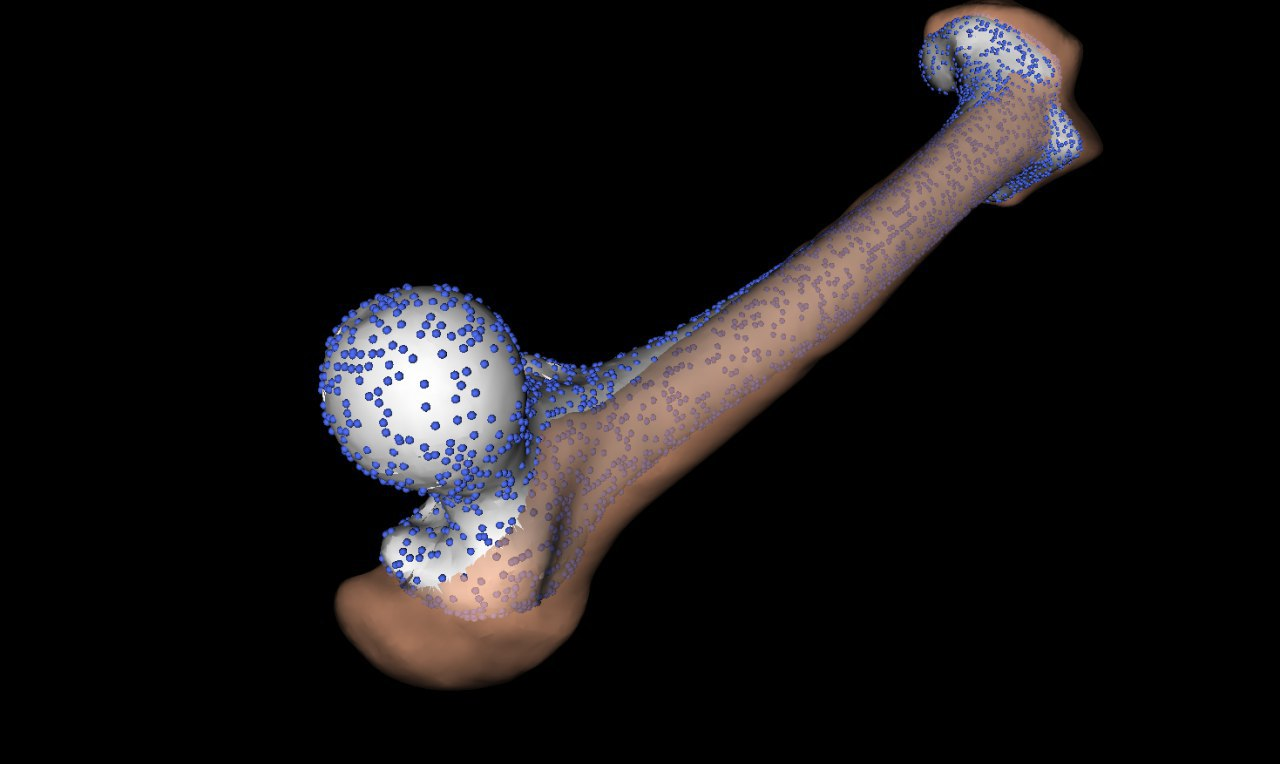
\includegraphics[width=7.3cm]{1.jpg}
		\caption{Uniformly sampled points on the mean of the SSM}
		
		\label{1.1}
	\end{subfigure}	
	\begin{subfigure}{.5\textwidth}
		\centering
		 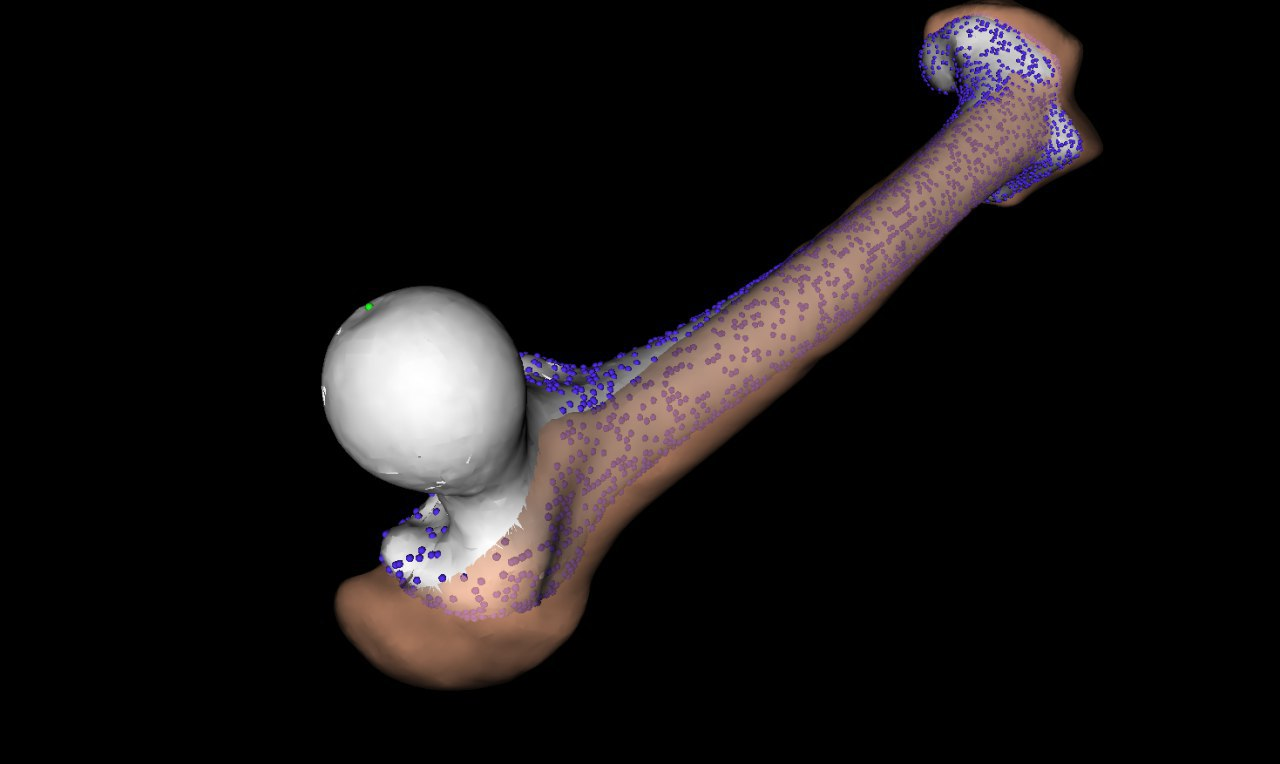
\includegraphics[width=7.3cm]{2.jpg}
		\caption{Filter applied on the sampled points}
		\label{1.2}
	\end{subfigure}	
	\end{figure}
	
	The regression that is done in each iteration finally leads to the reconstructed femur. But as some of the corresponding points do not exist on the partial femur bone, it is necessary to discard all points that can’t be mapped anywhere on the target mesh. This was done by designing individual filters for each partial femur. 
	Our main approach for the filtering was defining possible ranges for the z values and removing points that are in a certain radius around a selected point in the 3D space. \autoref{1.1} and \autoref{1.2} show the resulting sampled points for applying this method on the first femur. For the third femur we approximated the cutoff plane and discarded all points that are on the wrong side of this plane (see \autoref{2}).
	This method has the advantage, that we don't have to manually select correspondent points on the femurs but rather just define and exclude the area on our Shape Model that is missing in the target femur.
	
	
	\begin{figure}
	\centering
	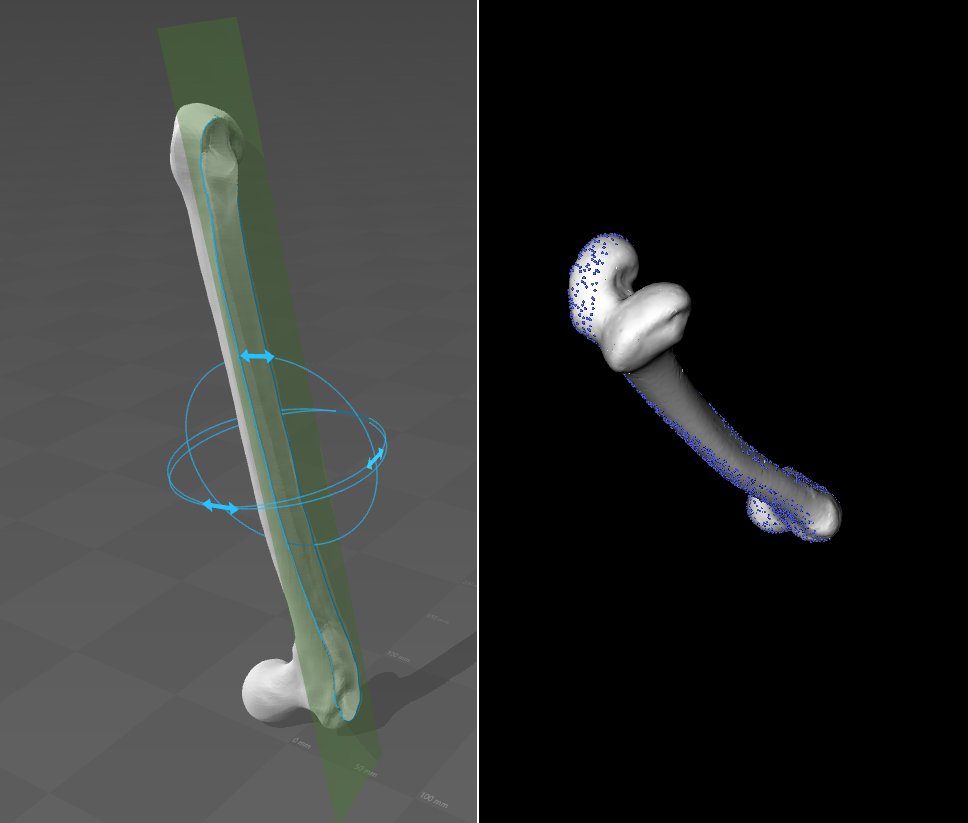
\includegraphics[width=10cm]{4.png}
	 \caption{ a) The missing area is best explained by a plane. 
	 	b) Sampled points on the mean shape after filtering with the estimated plane.}
	 \label{2}
	\end{figure}
	
	



	
	\section{Results \& Discussions}
	
	In \autoref{3} the average distance and the Hausdorff distance to the groundtruth of the missing part are listed. For the most part our method resulted in good reconstructions. The seventh and tenth partial femur stand out with a relatively high Hausdorff distance. A more accurate selection of landmarks may be necessary for a satisfying result. 
	For the different reconstructions we used both the augmented SSM as well as the SSM which was purely learned from the data. In terms of the average distance and Hausdorff distance we could not determine which one of the model is better in general. But the augmented model is less prone to unusual deformations and results in smoother shapes.
	\begin{figure}
		\centering
		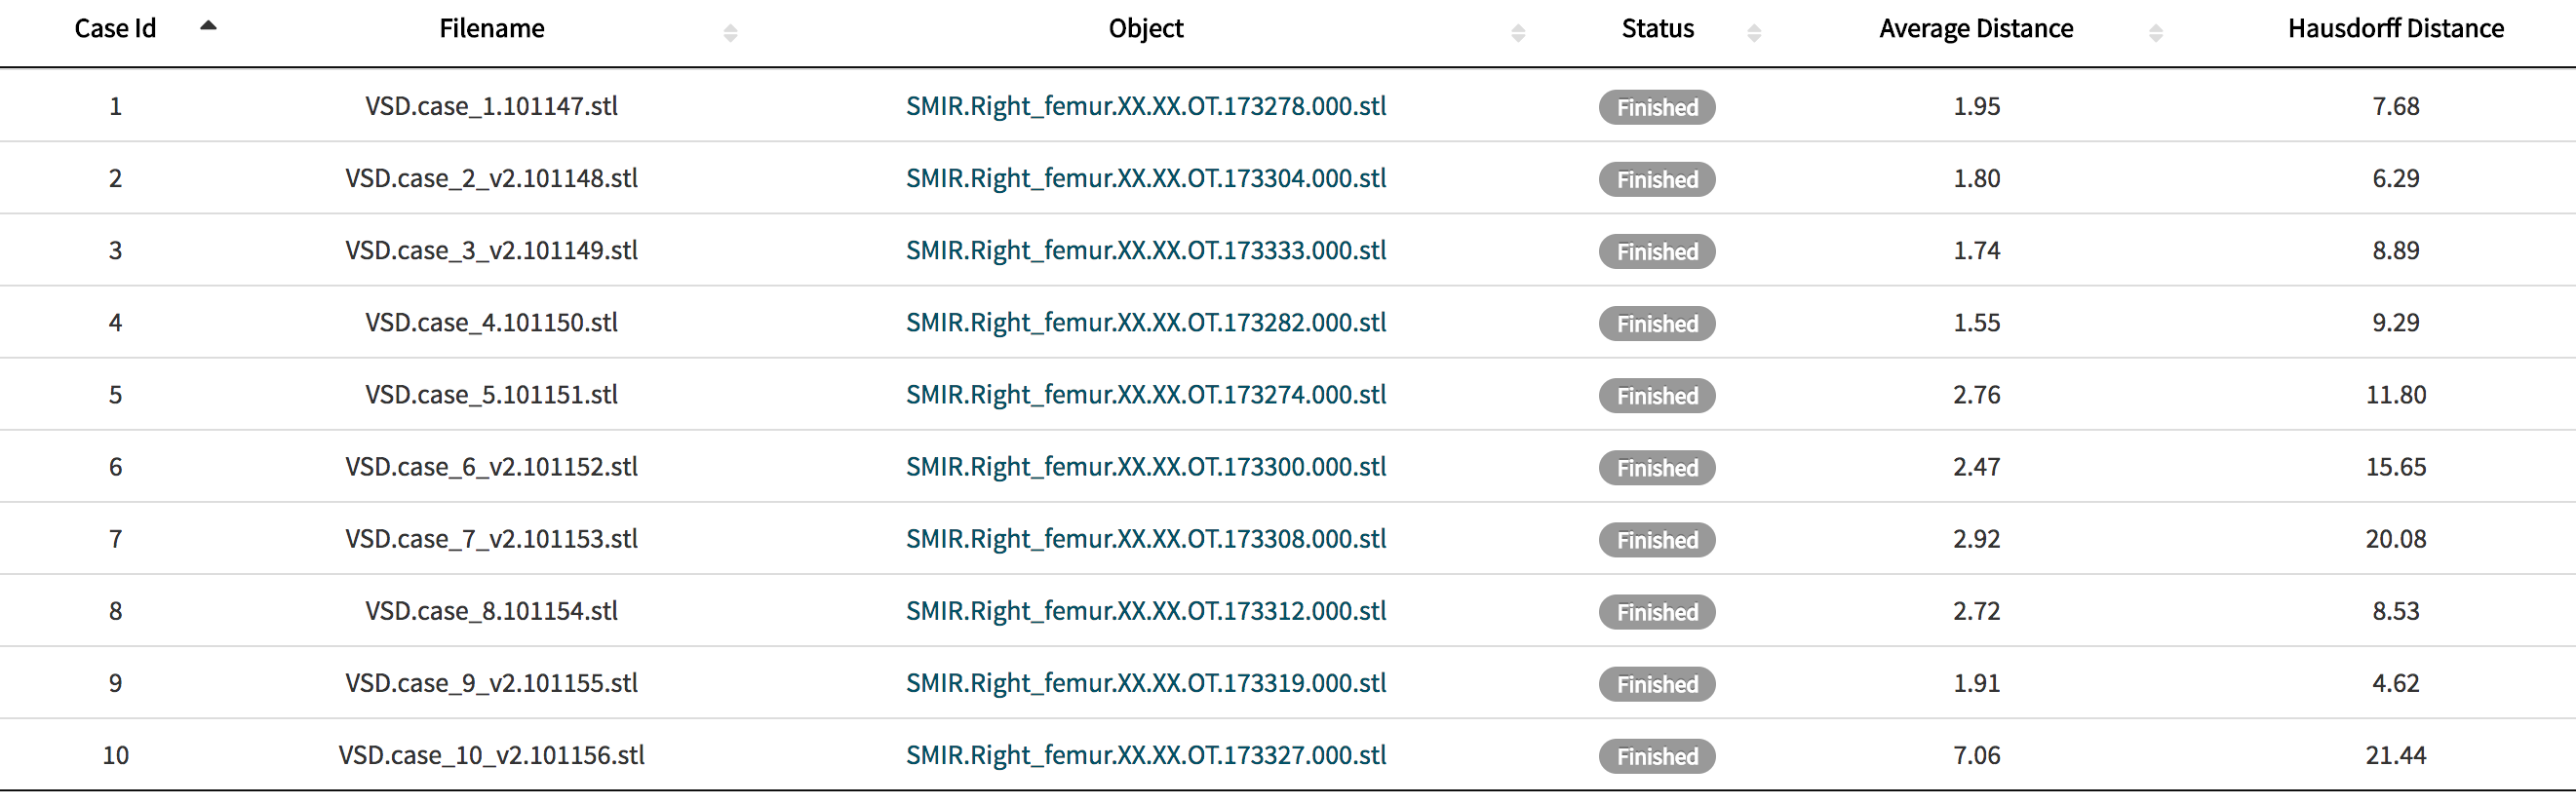
\includegraphics[width=15cm]{3.png}
		\caption{Reconstruction results}
		\label{3}
	\end{figure}

	Improvement of our methods could be achieved at three different steps of the reconstruction procedure. First of all, we could improve the SSM by using more elaborate methods for finding correspondence between the training femurs. Instead of initializing the ICP with the closest points to the sampled point, the provided landmarks could be used for the first regression. Aside from that, different algorithms than the ICP (e.g. gradient based approaches) may further improve the correspondence. Secondly, the data trained model can be further augmented with customly created kernels. At last, the reconstruction itself may benefit from additional use of manually selected landmarks for the ICP. 
	


\end{document}